\documentclass{acm_proc_article-sp}
\newcommand\floor[1]{\lfloor#1\rfloor}
\newcommand\ceil[1]{\lceil#1\rceil}
\newcommand{\tabitem}{~~\llap{\textbullet}~~}
\usepackage{textcomp}
\usepackage{url}
\usepackage{algorithm}% http://ctan.org/pkg/algorithms
\usepackage[noend]{algpseudocode}
\usepackage{pifont}
\usepackage{tabulary}
\usepackage{amsmath}
\usepackage{subcaption}
\usepackage{float}
\usepackage{cleveref}
\captionsetup{compatibility=false}

\begin{document}

\title{Who to query? \\A two step querying technique for tracking real-time variant/unknown event distributions }
\numberofauthors{3} %  in this sample file, there are a *total*

\author{
% You can go ahead and credit any number of authors here,
% e.g. one 'row of three' or two rows (consisting of one row of three
% and the second row of one, two or three).
%
% The command \alignauthor (no curly braces needed) should
% precede each author name, affiliation/snail-mail address and
% e-mail address. Additionally, tag each line of
% affiliation/address with \affaddr, and tag the
% e-mail address with \email.
%
% 1st. author
\alignauthor
Mai ElSherief\\
      \affaddr{Dept. of Computer Science }\\
      \affaddr{UC Santa Barbara}\\
     %\affaddr{Santa Barbara, CA}\\
      \email{mayelsherif@cs.ucsb.edu}      
      \alignauthor
Ramya Raghavendra\\
      \affaddr{IBM T. J. Watson Research Center }\\
      \email{rraghav@us.ibm.com}
% 2nd. author
\alignauthor
Elizabeth Belding\\
     \affaddr{Dept. of Computer Science }\\
      \affaddr{UC Santa Barbara}\\
      %\affaddr{Santa Barbara, CA}\\
      \email{ebelding@cs.ucsb.edu}
}

\maketitle


\begin{abstract}
Some abstract sentences...

\end{abstract}
%\category{H.1.2}{User/Machine Systems}{Human information processing}
%\keywords{Street harassment, Urban analysis, Walkability score, Transit Score, Transit route }


\section{Introduction}

Some introductory sentences...
%In particular, we seek to understand different harassment aspects, such as the location of events and the properties of these locations, so that this information can be used to inform prevention of future events.

\section{Related Work}
- Spatial task distribution (maximizing task assignment)\\
- Applications: emergency scenarios, safety applications, etc. 
- crowd sourcing and crowd sensing

\section{Research question and proposed technique}
In this paper, we envision a world where users can be probed to contribute to an unanswered question. An unanswered question can be related to a phenomenon that needs to be tracked under  constraints of $N$ resources. Examples include disastrous and safety applications. In particular, we have a two-dimensional grid and a number of objects that can sense the environment around them. These objects can be humans, artificial sensors, mobile phones or even robotic sensors. If we are interested in answering the question "How are things going in this grid?", we can basically ask or query all the objects in the two-dimensional space and aggregate their findings. In this paper, we assume that to answer this question, you can only query $N$ objects. Hence, the question becomes: \textit{Given $N$ resources, who should you select to track a real-time phenomenon?} Answering this question becomes essential in the case of a limited bandwidth of resources. This is particularly important in emergency scenarios when a network's performance degrades and preserving energy and other resources become important.\par
If we attempt to tackle this question from a probabilistic point of view, then the straightforward answer would be to try to select objects/users with the same probabilistic distribution as the phenomenon. For instance, if we know that a certain phenomenon occurs at different places in the two-dimensional grid uniformly, then we would have no bias in selecting the users to query i.e. each user/object would have the same probability of being selected to be queried. On the other hand, if we know the phenomenon we are interested in is more prevalent in certain areas of the grid as opposed to other areas, we would take that into consideration when we are selecting the users and select more users to query in this area and fewer users in other areas where there is a smaller probability of occurrence.\par
But what if you do not know the distribution or what if the distribution of the phenomenon is time variant? The aforementioned question becomes more interesting in this case and we can then inquire if there is a systematic algorithm that can be used for querying/selecting users to track a phenomenon regardless of the probabilistic distribution or time variations. \par
In this paper, we introduce a two-stage technique that can be used to select $N$ users to track a real-time phenomenon with no prior information about the event distribution. The technique outperforms the random user selection by a percentage of $20-63\%$ on average in terms of number of users chosen that were close in the events and outperforms the dispersion maximization technique by a percentage of $20-68\%$ on average.\par

\subsection{Technique Description}
We assume that we have $M$ users in our two-dimensional grid and that the system that selects a user to query is bounded by $N$ resources where $N < M$.  Each of the $M$ users has a specific location in the grid determined by a two-dimensional system e.g. (x, y) or a (lat, long). We also assume that the users selected will participate in answering the question of interest to the system and fully co-operate. A pre-selection phase can be used to eliminate users that aren't likely to co-operate or users who can provide false information using a system of building trust over time. The ways to rule out users based on trust or refusal to co-operate is not the main focus of this paper. Instead, we focus on how to select $N$ out of $M$ users to  where $N < M$ to keep track of events occurring in the two-dimensional grid.\par
Our technique combines $K$ nearest neighbor (KNN) queries with querying users to maximize the dispersion of their location in the grid as depicted in Algorithm 1. We devise the selection of users into two stages. In the first stage, our goal is selecting users with the aim of maximizing the dispersion of their locations. Based on the crowd feedback in the first stage, we go into a more fine-grained selection. The users that provide a positive feedback (i.e. they witness an event/ emergency in their location) are called the pivot users. In the second stage, we aim to get the $K$ nearest neighbors for the pivot users. We assume that because the pivot users witness an event, the $K$ nearest neighbors will probably witness another event of the same type in a neighboring area. \par
The aforementioned technique assumes full trust in the first stage users to respond and provide unfalsified responses. To remedy that, we can explore dividing the selection of the second phase users into two groups: a group comprising of the $KNN$ of the pivot users and another group that aims to maximize the dispersion. In this section, we will focus on studying our two-stage querying technique with the assumption of having full trust in the crowd and discuss other variants of the technique in subsequent sections.\par  
\begin{algorithm}
\caption{Two-stage querying algorithm}
\label{TSalgorithm}
    \begin{algorithmic}[1]
        \Function{selectUsersFromGrid }{$FSP, N$}
            \State selectedUsers = $\left\{\right\}$
            \State firstStageCnt = $\floor{(FSP*N)}$
            \State secondStageCnt = $M - firstStageCnt$
            \State firstStageUsers = maximizeDisp(firstStageCnt)
            \State usersFeedback = feedback(firstStageUsers)
            \If {usersFeedback.size == 0}
                   \State selectedUsers = maximizeDisp(secondStageCnt){}
            \Else
                \State {selectedUsers.append(firstStageUsers)}
            \EndIf    
          \State firstStageQuota = calculateQuota(firstStageUsers)
          \For{$user_i$ in firstStageUsers}
        \State selectedUsers.append(KNN($user_i$, $firstStageQuota_i$))
      \EndFor
\State return {selectedUsers}
\EndFunction
\end{algorithmic}
\end{algorithm}

\section{Expermients}
In order to quantify the performance of our technique, we test it under different scenarios. We investigate the technique using three types of data spread: clustered, uniform and real datasets. In our experiments, we compare our algorithm in the selection of users to two policies as follows.
\begin{itemize}
\item Random user selection: For this policy, we select $N$ users randomly based on a uniform distribution.
\item Selection based on dispersion maximization: The selection of users in this policy depends on selecting $N$ users from the crowd who maximize the dispersion of their locations.
\end{itemize}
\subsection{Experiments Variables}
There are multiple variables that can be controlled to test the behavior of the two-stage querying technique. Table~\ref{table:systemParameters} explains the most important variables.


\begin{table}{}
\centering
\begin{tabulary}{0.5\textwidth}{|L|}
\hline
\textit{Environment settings: }\\
\tabitem matrix dimension: represents the length and 
the width of the $2D$ spatial matrix. We model the spatial area under investigation as a $2D$ square matrix.\\
\tabitem incident count: number of incidnets distributed across the cells of the spatial matrix\\
\tabitem resources or crowd count: the $M$ resouces from which $N$, where $N < M$, will be chosen to query\\
\hline
\textit{Query settings:}\\
\tabitem $N$: the number of resources the system is limited by to query/sense \\
\tabitem first stage percentage (FSP): the percentage of users/sensors of the $N$ resources that will be selected to query in the first phase. In our analysis, we test the cases of selecting $20\%, 40\%, 60\%$ and $80\%$ of the $N$ resources in the first stage.\\
\tabitem k setting: used to identify the KNN crowd individuals/sensors to an incident\\
\hline
\textit{Approximation settings: }\\
\tabitem Maximization trials: number of attempts to maximize the dispersion of selected individuals/sensors from the crowd\\
\hline
\end{tabulary}  
\caption{Different parameters of the two-stage querying technique.}
\label{table:systemParameters}
\end{table}

The environment settings are related to the size of the $2D$ matrix, the number of incidents and their distribution across the matrix and the number of resources to choose from. In all of our experiments, except the case study, we set up the $2D$ matrix as a $10$ by $10$ matrix. We show results for incident count of $50$ and  number of resources or $M$ of $100$. We varied the environment settings in our experiments and no noticeable differences were observed in performance. Instead, we focus on varying the query settings to better understand the two-stage technique. In this section, we will focus on varying the first stage percentage and leave the variation of the $k$ setting to the following section. We also show results for $t\_setting = 30$ which constitutes $30\%$ of the available resources ($M$). We notice that the gap between the performance of our technique and the other techniques increase when $t\_setting$ decreases and all the techniques converge in performance when $t\_setting$ approaches $M$. \par
  
 To measure the performance of our technique in comparison to other forms of selection, we utilize two different metrics namely count of people/sensors queried in the $KNN$ of incidents and the number of incidents covered by the people queried. The two metrics are formally defined as follows.
 \begin{itemize}
 \item Close people count: This is measured as the absolute number of people/resources in the KNN of each incident for all incidents. This is formally represented as follows:
 \begin{equation}
 Close\ people\ count = \sum \forall_{incident\ i}\ |(KNN_i \cap {QU})|
 \end{equation}
 where $QU$ (the ``Queried Users'' set) is the set of users selected for querying. 
 \item Coverage: measured as the number of incidents covered out of the total number of incidents occurring in the $2D$ matrix. We define an incident to be covered if at least one of the people/resources in the incident's KNN was queried. This is formally measured as:
 \begin{equation}
Coverage = \sum \forall_{incident\ i}\ Coverage_i\  where,
 \end{equation}
 \[
    Coverage_i = 
\begin{cases}
    1,& \text{if }(KNN_i \cap {QU}) \neq \phi\\
    0,              & \text{otherwise}
\end{cases}
\]
\end{itemize}  

\subsection{Clustered data experminets}
In this subsection, we aim to test our technique in a scenario where the events take a clustered form. Geographer Waldo R. Tobler's stated in the first law of geography: ``Everything is related to everything else, but near things are more related than distant things.'' In this subsection, we assume that the incidents are related to each other and that they take a clustered form i.e. they form clusters across the $2D$ spatial matrix as seen in Fig~\ref{fig: clust}. \par
\begin{figure}[!h]
\centering
   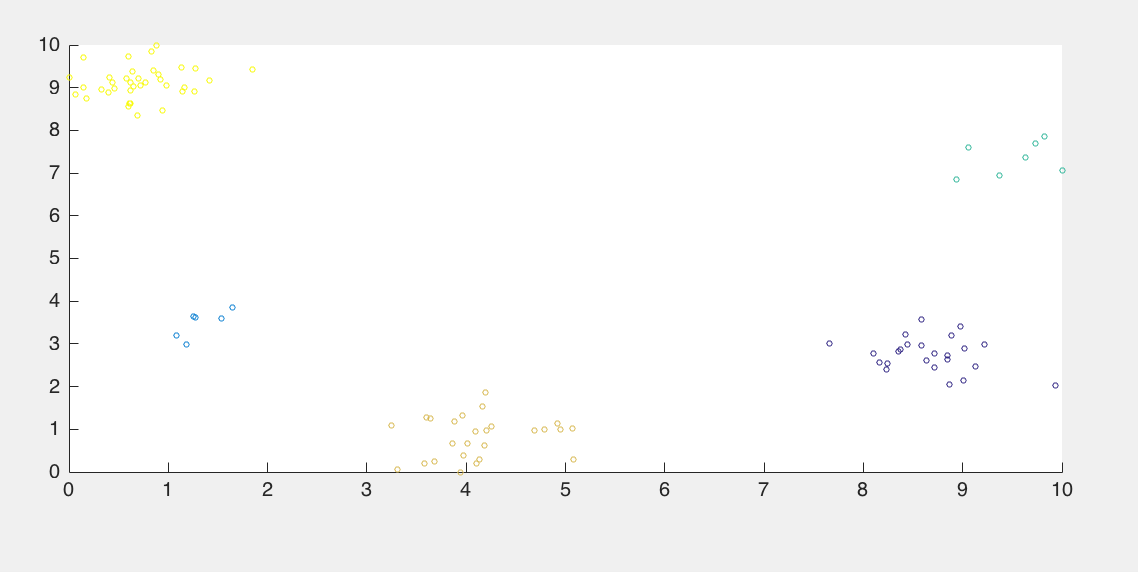
\includegraphics[width=9cm ,height=5.5cm]{figuresPng/clust.png}
   \caption{An example of a $2D$ spatial matrix with $5$ clusters }\label{fig: clust}
\end{figure}
For these type of experiments, we vary the number of clusters in our $2D$ matrix from one cluster to ten clusters while fixing the resources or crowd count to be $100$. To ensure data variability, we model the size of each cluster as a random variable while making sure that the aggregated size of all the clusters is equal to the crowd count. For each case of varying the number of clusters, we average over $100$ different configurations. The objective in this section is to measure the effect of variation of the first stage percentage on our performance metrics.\par
Figures~\ref{fig:clusteredResults}\subref{fig: clust_20},~\ref{fig:clusteredResults}\subref{fig: clust_40},~\ref{fig:clusteredResults}\subref{fig: clust_60},~\ref{fig:clusteredResults}\subref{fig: clust_80} depict the results for Close People count when varying the first stage percentage from $20\%$ to $80\%$. We notice that our two-stage querying technique always outperforms the Random crowd/sensors selection and the selection based on maximizing the dispersion only. Table~\ref{table:clusteredSurge} depicts the amount of surge in Close people count in comparison to Random and Dispersion Maximization techniques. We notice that as the amount of resources queried in the first stage decreases, the number of close people queried increases. This is due to the fact that when the first stage percentage decreases, the second stage resources increase under limited resources constraints which focuses on resources close to incidents detected in the first stage. On the other hand, incident coverage tends to increase as the first stage count increases. This is depicted in Figure~\ref{fig: clustCoverage}. We can also notice that both Close people count and Incident coverage tends to increase with the number of clusters till the number of clusters is around four or five and then decreases.

\begin{table}[!h]
\centering
\begin{tabulary}{0.5\textwidth}{|C|C|C|C|C|}
\hline 
 First stage percentage & $20\%$ & $40\%$  & $60\%$  & $80\%$  \\ \hline
Surge over Random   & $62.5\%$ & $58.89\%$  & $35\%$  & $20\%$  \\ \hline
Surge over Dispersion Maximization   & $67.8\%$ & $62.32\%$  & $39.8\%$  & $20.64\%$ \\ \hline
\end{tabulary}  
\caption{Surge of Two Stage technique in comparison to Random and Dispersion Maximization techniques.}
\label{table:clusteredSurge}
\end{table}
 

%Real life examples of clustered events include 
%- Begin by pointing out real-life examples of spatially clustered phenomenon and spatial correlation in general. Lots of social phenomena are spatially dependent. %(https://books.google.com/books?id=jbFRojt85TUC&pg=PA2&lpg=PA2&dq=clustered+phenomena&source=bl&ots=yftMfShveB&sig=XcPOJriI1gineu-%A2YGpoJT3OII&hl=en&sa=X&ved=0ahUKEwiBp4a-s-zKAhUI5WMKHZQ3Cd8Q6AEITzAI#v=onepage&q=clustered%20phenomena&f=false)

\begin{figure}[!h]
\centering
\subcaptionbox{Average number of people close to the incidents (Close people count) when maximizing the dispersion with $20\%$ of available resources. \label{fig: clust_20}}{%
  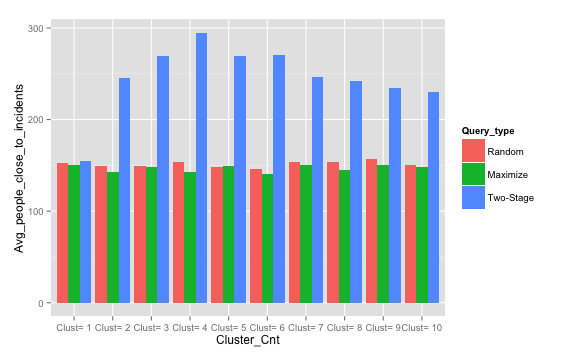
\includegraphics[width=9cm, height=4.5cm]{figuresPng/fsTwentyPerc.png}%
  }\par\medskip
\subcaptionbox{Average number of people close to the incidents (Close people count) when maximizing the dispersion with $40\%$ of available resources.\label{fig: clust_40}}{%
  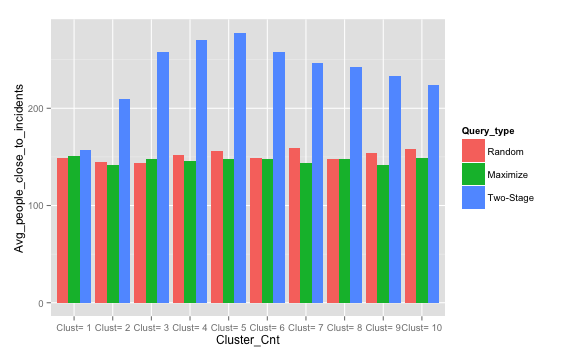
\includegraphics[width=9cm, height=4.5cm]{figuresPng/fsFourtyPerc.png}%
  }\par\medskip        
\subcaptionbox{Average number of people close to the incidents (Close people count) when maximizing the dispersion with $60\%$ of available resources.\label{fig: clust_60}}{%
     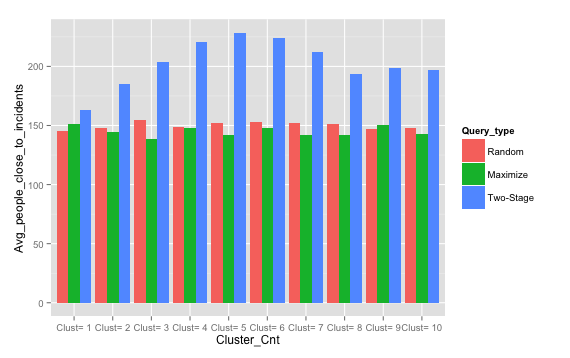
\includegraphics[width=9cm ,height=4.5cm]{figuresPng/fsSixtyPerc.png}%
  }
  \subcaptionbox{Average number of people close to the incidents (Close people count) when maximizing the dispersion with $80\%$ of available resources.\label{fig: clust_80}}{%
     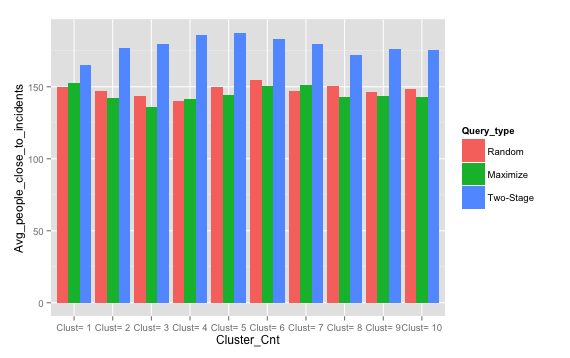
\includegraphics[width=9cm ,height=4.5cm]{figuresPng/fsEightyPerc.png}%
  }
\caption{Varying the first stage percentage with different number of clusters.}
\label{fig:clusteredResults}
\end{figure}

\begin{figure}[!h]
\centering
   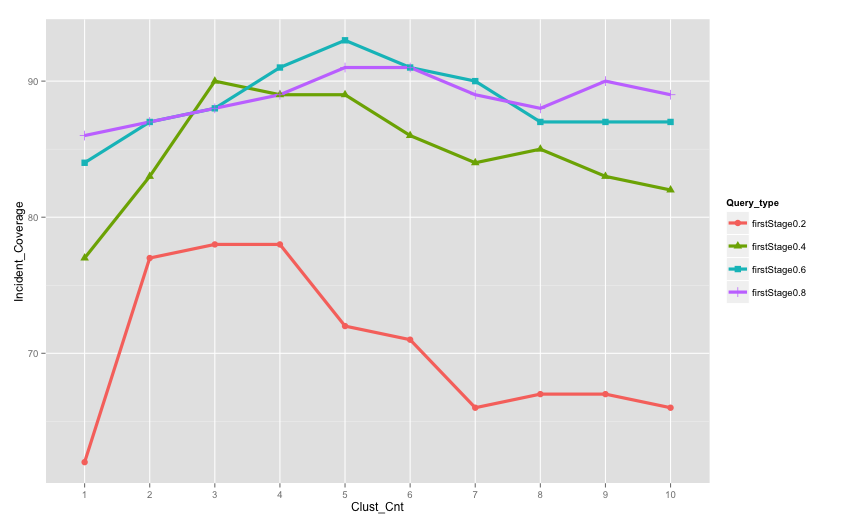
\includegraphics[width=9cm ,height=5.5cm]{figuresPng/Coverage_Result.png}
   \caption{Incident coverage for different values of First stage percentage. }
   \label{fig: clustCoverage}
\end{figure}



\subsection{Uniformly distributed data experiments}
- put uniformly distributed results here


\subsection{Long Tail Distribution}
- put long tail results here

\subsection{Case Study: Hollaback harassment data set}
After applying the two-stage querying technique to the previously mentioned three distributions (clustered, uniform and long-tail), we wish to examine the technique under real incident distributions. In order to do that, we test our querying technique on a global street harassment dataset provided by Hollaback~\cite{hollaback}.

\subsubsection{Data Overview}
Hollaback~\cite{hollaback} is a non-profit movement powered by local activists in $92$ cities and $32$ countries to end street harassment. The Hollaback project collects data on street harassment events worldwide. Through the Hollaback phone app and the online platform, users can report stories of street harassment to share with the Hollaback community. This empowers victims to speak out about everyday harassment and spread the word about the prevalence of these events. In some communities, local governments are informed in real-time about street harassment so that there is a system-wide level of accountability. In addition, the Hollaback app uses GPS to record a data set representing the locations of street harassment events as a means of improving the collective understanding of street harassment and how it can be prevented.  As of January $2016$, over $8000$ street harassment incidents have been recorded in their dataset since February $2011$.  It is on this data set that we wish to test the two-stage querying technique.\par
\subsubsection{Analysis}
Going through the Hollaback dataset, we select different cities for which we have enough harassment samples for statistical significance (i.e. more than 30 samples). We test the performance of Random selection, Dispersion maximization selection, and the two-stage querying on six different cities: Paris in France, Brussels in Belguim, Berlin in Germany, Baltimore, Maryland in the US, Buenos Aires in Argentina and Istanbul in Turkey. In this paper, we show results for Paris, Brussels and Istanbul. \par

In order to separate the collected Hollaback dataset into different cities, we used bounding box coordinates. After that, we drew the border lines for the different cities and removed any outliers from our datasets. Figure~\ref{fig:citiesDistribution} shows the distribution of events for the different cities. The Paris dataset contains $197$ harassment incidents and covered an area of $28.2$ sq mi while the Brussels dataset contains $154$ incidents covering a geographic area of $28.4$ sq mi. Istanbul had $87$ reported incidents covering an area of $138$ sq mi on the left of Bosporus Strait and $69$ sq mi on the right. \par

\begin{figure}[!h]
\centering
\subcaptionbox{Hollaback harassment reports in Paris. \label{fig: clust_20}}{%
  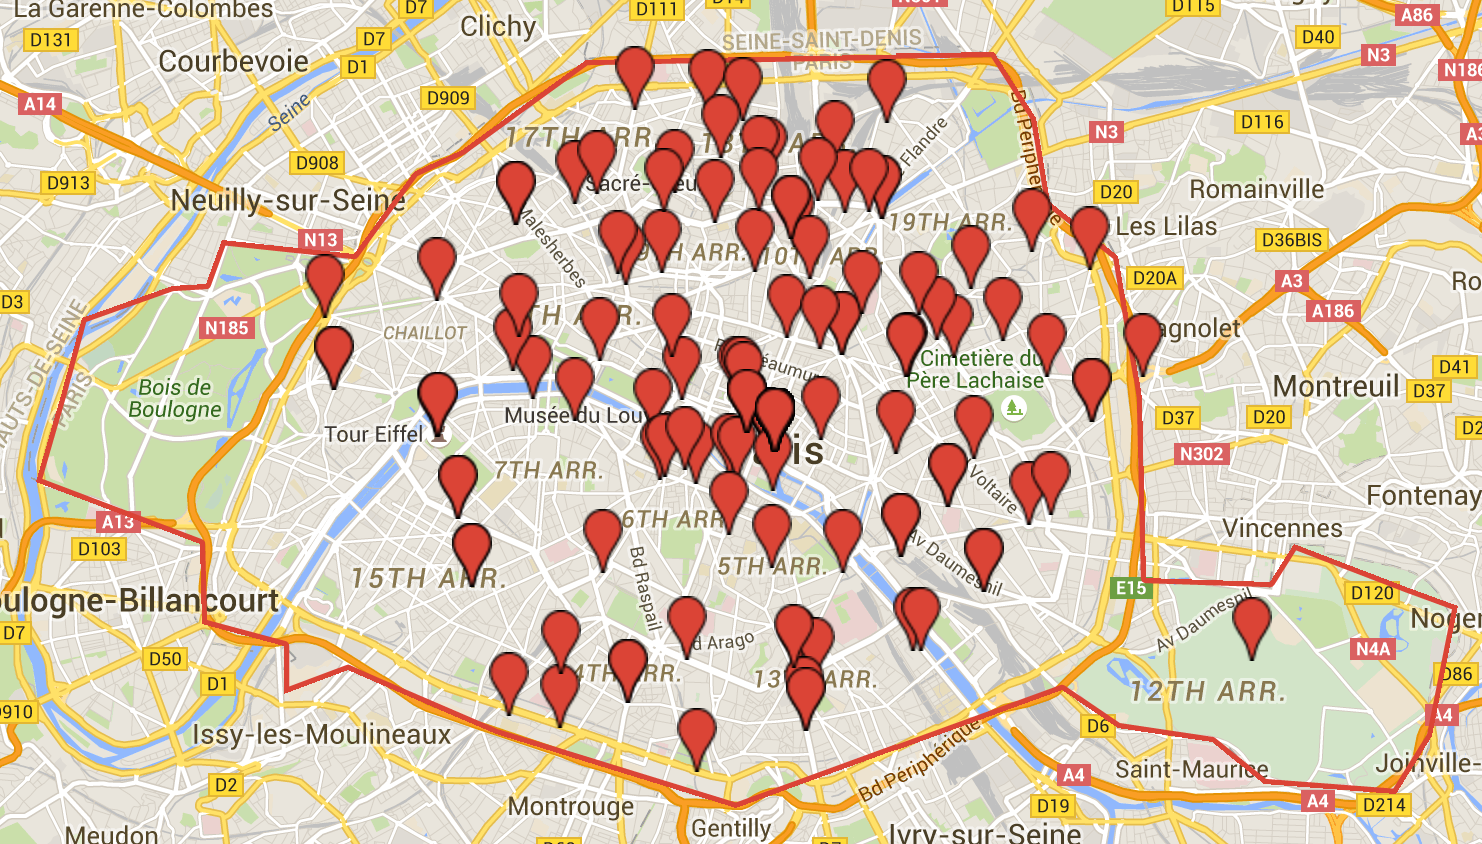
\includegraphics[width=8cm, height=5cm]{figuresPng/Paris.png}%
  }\par\medskip
\subcaptionbox{Hollaback harassment reports in Brussels.\label{fig: clust_40}}{%
  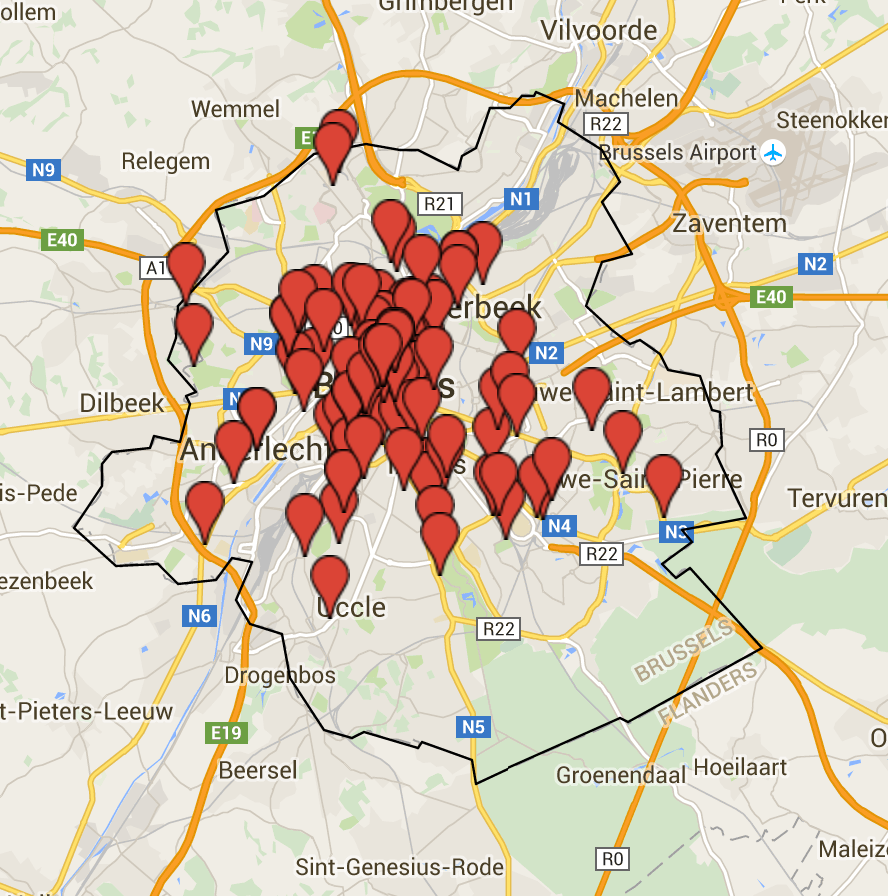
\includegraphics[width=8cm, height=5cm]{figuresPng/Brussels.png}%
  }\par\medskip        
\subcaptionbox{Hollaback harassment reports in Istanbul.\label{fig: clust_60}}{%
     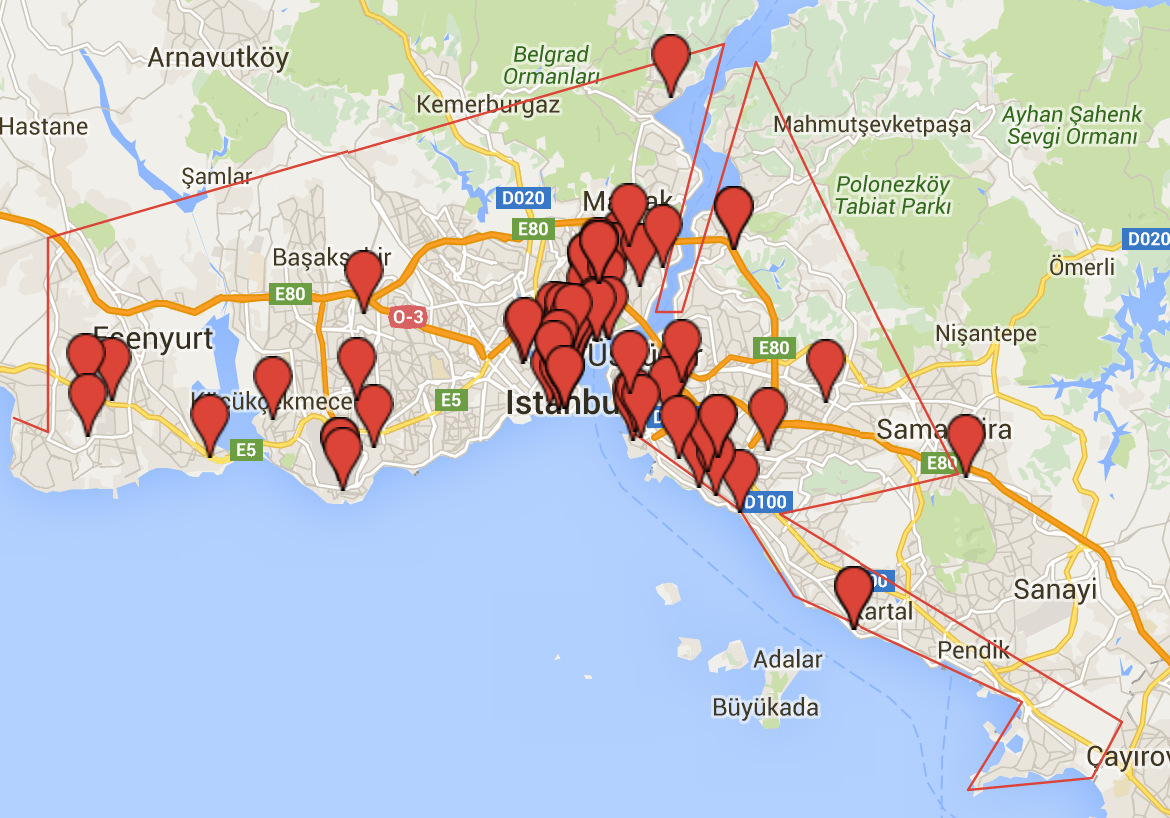
\includegraphics[width=8cm ,height=5cm]{figuresPng/Istanbul.png}%
  }
\caption{Distribution of harassment incidents across Paris, Brussels and Istanbul.}
\label{fig:citiesDistribution}
\end{figure}

For each of the cities, we generate different variations of uniformly distributed crowd ($M = 100$) across the city. In this kind of analysis the parameters, matrix dimension and incident count, are not controlled by our analysis but rather enforced by the dataset. We measure the Close people count and the Incident Coverage for all three querying techniques and plot the results in Figure~\ref{fig: hollaCloseCount} and Figure~\ref{fig: hollaIncCoverage} respectively. We notice that the Two-stage technique outperforms both the Random and Dispersion Maximization in terms of Close People count for all three cities. In terms of incident coverage, Figure~\ref{fig: hollaIncCoverage} shows that dispersion maximization achieves maximum incident coverage. The figure also shows that the two-stage technique can achieve this maximum by setting the first stage percentage to be $80\%$. The aforementioned two figures suggest that there is an inherent tradeoff between accuracy and coverage under constrained resources which we will discuss in detail in later sections. The figures also suggest that the two-stage technique under setting the first stage percentage to be $80\%$, can achieve a balance between accuracy and coverage.



\begin{figure}[!h]
\centering
   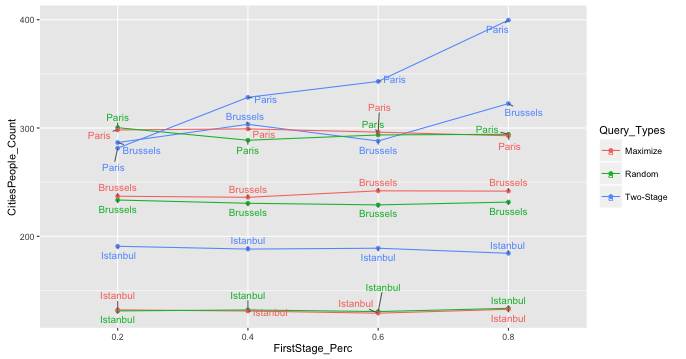
\includegraphics[width=9cm ,height=5.5cm]{figuresPng/hollaCloseCnt.png}
   \caption{Close people count for different values of First stage percentage. }
   \label{fig: hollaCloseCount}
\end{figure}
\begin{figure}[!h]
\centering
   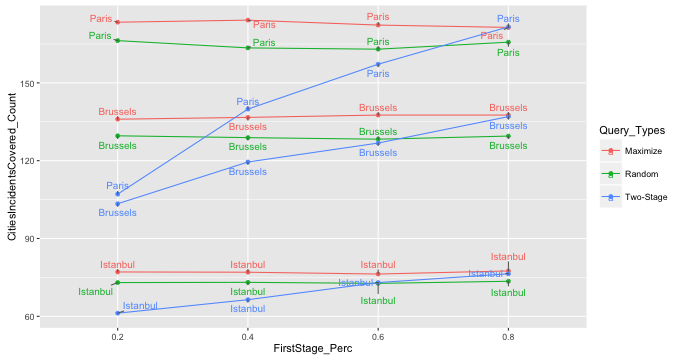
\includegraphics[width=9cm ,height=5.5cm]{figuresPng/citiesInc.png}
   \caption{Incident coverage for different values of First stage percentage. }
   \label{fig: hollaIncCoverage}
\end{figure}


\subsection{Stressing the two stage querying technique (k=1)}
\subsection{Technique Variations}
- prior knowledge variation
- second stage division
\section{Discussion}
- Our assumptions and limitations...

\section{Conclusions}
In this paper, we introduced.... 

\section{Acknowledgments}

\bibliographystyle{abbrv}
{\footnotesize
\bibliography{sigproc}}  % sigproc.bib is the name of the Bibliography in this case
% You must have a proper ".bib" file
%  and remember to run:
% latex bibtex latex latex
% to resolve all references
%
% ACM needs 'a single self-contained file'!
%
%APPENDICES are optional
%\balancecolumns



\end{document}